\subsection{Ablation Study}

% 1. Ablation on the debug step over three models on alfoworld test 100, gpt-4o-mini, qwen3-8b, qwen3-next-80b

% 2. Ablations on the different dection models

% 3. ablations on different rollout method:REACT REFLEXION, ACT ONLY, WITH MEMORY


To better understand the contribution of each component in our framework, we conduct a series of ablation studies. Specifically, we analyze the following factors.

\noindent{\textbf{Max Number of Attempts Allowed.}}  
We vary the maximum number of attempts of \ModelName{} with different base models— GPT-4o-mini, Qwen3-8B, and Qwen3-Next-80B—to examine how sensitive performance is to the chosen point of intervention. Results in Figure~\ref{fig:alfworld_success_rates} show that additional attempts yield consistent gains across all backbones, with especially pronounced improvements on smaller models such as GPT-4o-mini. This highlights the value of targeted re-rollouts in boosting task success.

\noindent{\textbf{\ModelName{} Base Models.}}  
We replace the base model of \ModelName{} with several alternatives to assess their impact on error localization and downstream success. As shown in Figure~\ref{tab:ablation_detector}, GPT-4.1 substantially outperforms other models, achieving 42\% step accuracy and 32\% strict all-correct accuracy. Competing base models such as Llama-3.3-70B, GPT-4o-mini, and Qwen3-Next-80B perform markedly worse.

\noindent{\textbf{Rollout Strategies.}}  
We compare several rollout paradigms—ReAct, Reflection, Act-only, and Memory+ReAct—against our proposed \textbf{Modular} strategy on Alfworld under the zero-shot setting. As shown in Table~\ref{tab:ablation_rollout}, \ModelName{}’s Modular rollout achieves the highest score (0.38), outperforming both reasoning-only and memory-augmented baselines. This result highlights the effectiveness of structured modularization is more reliably than alternative rollout designs.


\begin{figure}[htbp]
\centering

% --- Column 1: Plot ---
\begin{subfigure}{0.55\linewidth}
    \centering
    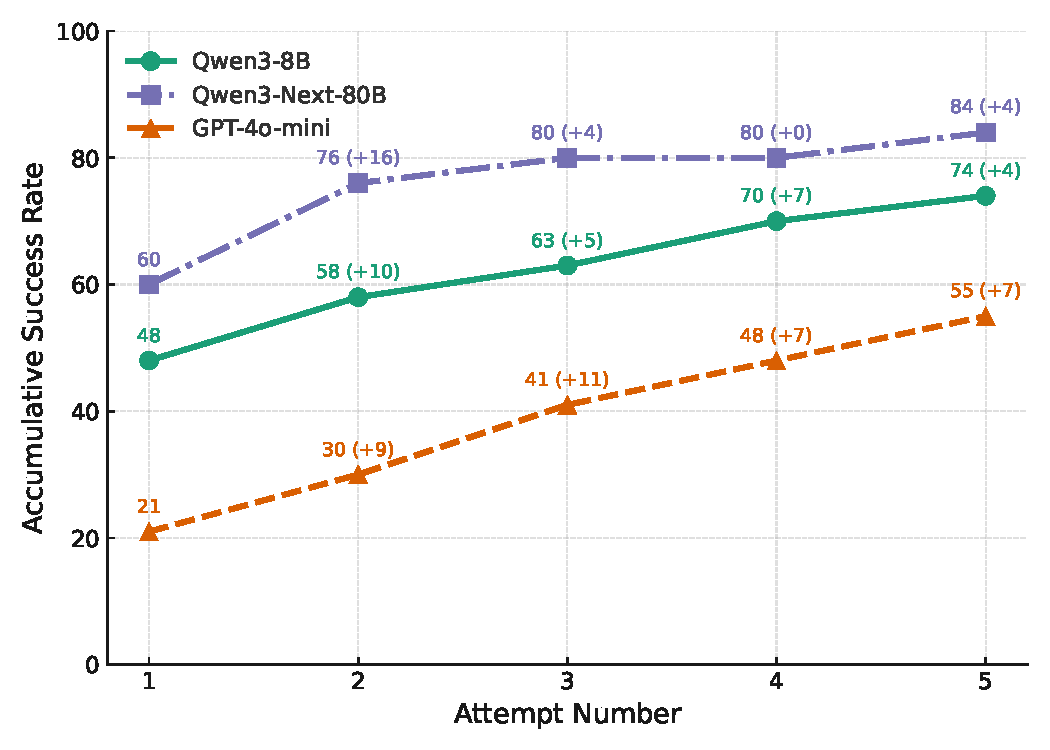
\includegraphics[width=\linewidth]{iclr2026/figures/task_success_rates_qwen_grouped.pdf}
    \caption{Success rates on Alfworld across five attempts.}
    \label{fig:alfworld_success_rates}
\end{subfigure}%
\hfill
% --- Column 2: Stacked Tables ---
\begin{subfigure}{0.45\linewidth}
    \centering
    
    % --- Subfigure B: Detector Table ---
    \begin{subfigure}{\linewidth}
        \centering
        \scriptsize
        \begin{tabular}{lcccc}
        \toprule
        \textbf{Base Model} & \textbf{Step} & \textbf{Error} & \textbf{Step+M} & \textbf{All} \\
        \midrule
        Llama-3.3-70B    & 16.0 & 16.0 & 6.0 & 2.0 \\
        GPT-4o-mini  & 14.0 & 10.0 & 4.0 & 2.0 \\
        Qwen3-Next-80B    &  4.0 & 14.0 & 2.0 & 2.0 \\
        \rowcolor{yellow!20}\textbf{GPT-4.1} & \textbf{42.0} & \textbf{44.0} & \textbf{32.0} & \textbf{32.0} \\
        \bottomrule
        \end{tabular}
        \caption{Base Model Performance Comparison.}
        \label{tab:ablation_detector}
    \end{subfigure}
    
    \vspace{0.5cm}
    
    % --- Subfigure C: Rollout Table (wider) ---
    \begin{subfigure}{1.1\linewidth} % make table C wider
        \centering
        \scriptsize
        \begin{tabular}{lc}
        \toprule
        \textbf{Rollout Strategy} & \textbf{Success Rate} \\
        \midrule
        Memory+ReAct & 0.34 \\
        Reflection   & 0.32 \\
        ReAct        & 0.26 \\
        Act Only     & 0.10 \\
        \rowcolor{yellow!20}\textbf{Modular} & \textbf{0.38} \\
        \bottomrule
        \end{tabular}

        \caption{Rollout Strategy Comparison.}
        \label{tab:ablation_rollout}
    \end{subfigure}
    
\end{subfigure}


\caption{Ablation study results. (a) Success rates on Alfworld, (b) comparison of detector models, and (c) rollout strategy analysis.}
\label{fig:ablation_combined}
\vspace{-0.1in}
\end{figure}

\subsection{Error Propagation}
\label{subsec:error_propoagate}

% Discussion over the error propagation, graphics and statistics
% some statistics by human and llm judge

% how often it cause the cascading effect(not always)

% how length it will cause the cascading effect

% which module and steps range cause the most of 

% some take away to prevent 

A key challenge in building robust LLM agents lies in understanding how small mistakes evolve into large-scale failures. Our analysis examines the phenomenon of error propagation—cases where an early misstep triggers a cascading effect that spreads throughout the trajectory. As shown in Figure \ref{fig:error_propagation},  early-stage mistakes cascade through later steps across tasks. The outlined cells indicate the first critical error in each trajectory, while progressively darker red shading reflects the compounding severity and persistence of errors over subsequent steps. This illustrates how initial failures frequently propagate forward, amplifying downstream task breakdowns.

\begin{figure}[ht]
    \centering
    \vspace{-8mm}
    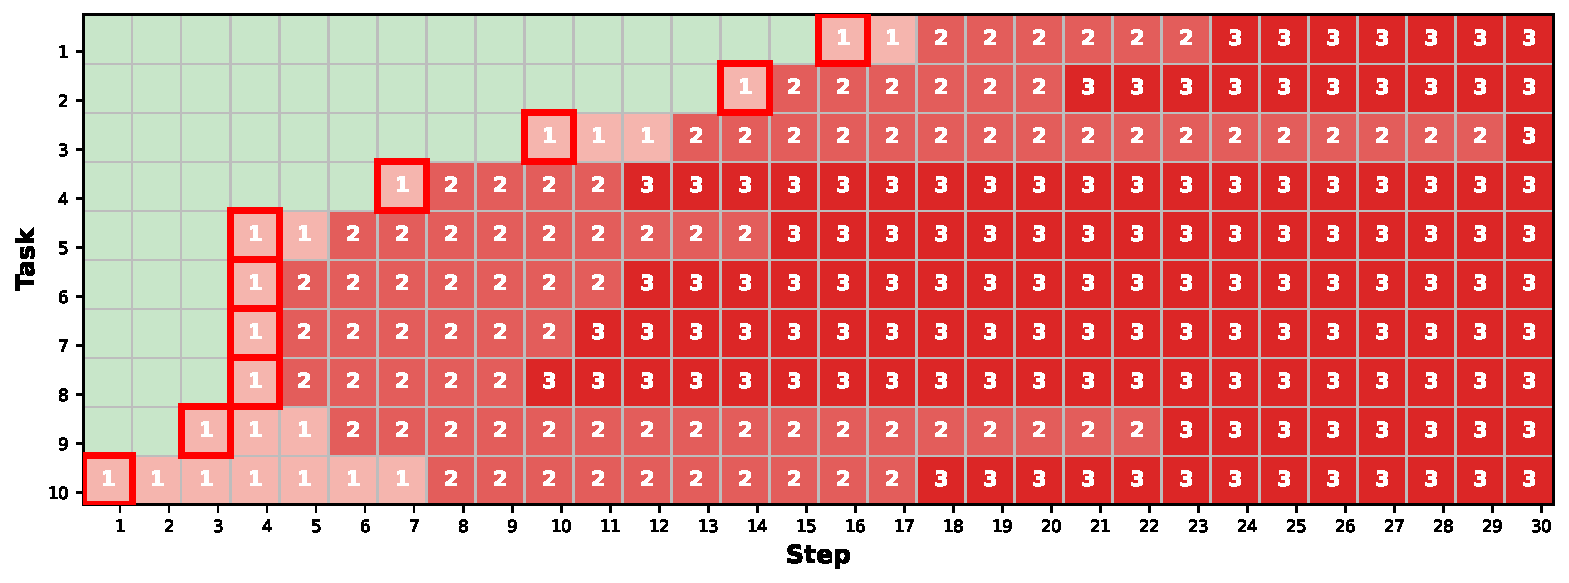
\includegraphics[width=1\linewidth]{iclr2026/figures/grid_10x30_levels.pdf}
    \caption{\textbf{\textit{Illustration of Error Propagation}}: Darker shading indicating compounding failures and highlighting how initial mistakes amplify downstream breakdowns.}
    \vspace{-0.20in}
    \label{fig:error_propagation}
\end{figure}

Moreover, the likelihood and length of cascades vary significantly across modules. Memory and reflection errors are the most common sources of propagation, typically arising in early or mid-trajectory steps (around steps 5–15). Once an agent misremembers a fact or misjudges its progress, subsequent planning becomes systematically distorted, leading to repeated cycles of flawed action selection. Planning errors also contribute heavily, with constraint ignorance or infeasible strategies compounding as the agent attempts to execute them. By contrast, action-level errors are more visible and sometimes recoverable, though malformed outputs or missing parameters can still derail execution. System-level issues such as tool crashes or step-limit exhaustion act as immediate termination points rather than cascades.

These findings highlight two important takeaways for designing more reliable agents. First, \textbf{early detection and correction are critical}, since once cascades begin, they are difficult to reverse. Second, mechanisms that strengthen memory retrieval and reflection—such as external memory, progress tracking, or verification prompts—can substantially reduce the risk of propagation.




% \subsection{Case Study}
% sucessful debug case and how it can evolve through 

% one more specific error propagation case

% Statistics on the error types and steps distribution on benchmarks


